\documentclass[]{article}
\usepackage[utf8]{inputenc}
\usepackage[left = 1.5cm, right = 1.5cm, top = 2cm, bottom = 2cm]{geometry}

\usepackage{graphicx}
\usepackage{float}
\usepackage{amsmath}
\usepackage{cleveref}
\title{RES}
\author{William Rooke\\12051342}
\date{\today}

\begin{document}

	%\begin{titlepage}
	\begin{center}
		\vspace*{1cm}
		
		\Huge
		\textbf{PV Measurement}
		
		\vspace{0.5cm}
		\LARGE
		48550 Renewable Energy Systems - Lab 1
		
		\vspace{1.5cm}
		
		\textbf{Robert Carey}\space\space\space99139382\\
		\textbf{William Rooke}\space\space\space 12051342\\
		\textbf{Joel Goodwin}\space\space\space 98055953\\
		
		\today
		
		\vfill
		
		
		\vspace{0.8cm}
		
		\includegraphics[width=1\textwidth]{uts}
		
		
		
	\end{center}
\end{titlepage}
	
	\section{Introduction}
	    

   	
   	\section{Constant Voltage Reference MPPT}
   	    \subsection{Pre-Work}
       	    \subsubsection{Explain the working principle of the PV emulator.}
    	        \begin{figure}[H]
    	        	\centering
    	        	\includegraphics*[width=0.75\textwidth]{Prework_images/PVDiagram}
    	        	\caption{Diagram of PV emulator and voltage control}
    	        \end{figure}
    	        It can be seen from the above diagram that
    	        \begin{equation}\label{eq:TotalCurrent}
    	            I_{pv} = I_{ph} - i_{Dpv} - i_p
    	        \end{equation}
    	        where the diode current $i_{Dpv}$ is given by
    	        \begin{equation}\label{eq:DiodeCurrent}
    	            i_{Dpv} = I_S (e^{\frac{V_D}{V_T}} - 1)
    	        \end{equation}
    	        and the thermal voltage of the diode $V_T$ is 
    	        \begin{equation}\label{eq:ThermalVoltage}
    	            V_T=\frac{K_B*T*A}{q}
    	        \end{equation}
    	        where A is the ideality factor of the solar cell, q is the charge of an electron, $K_B$ is the Boltzmann constant, T is the temperature in Kelvin and the voltage across the diode $V_D$ is
    	        \begin{equation}\label{eq:DiodeVoltage}
    	            V_D=V_{pv\_c}-I_{pv}*R_s
    	        \end{equation}
    	        The leakage current $I_p$ is given by
    	        \begin{equation}\label{eq:LeakageCurrent}
    	            i_p=\frac{V_{pv\_c}+I_{pv}*R_s}{R_{sh}}
    	        \end{equation}
    	        Combining \crefrange{eq:TotalCurrent}{eq:LeakageCurrent} gives the output current as
    	        \begin{equation}
    	            I_{pv}=I_{ph}-I_S(e^\frac{V_{pv\_c}-I_{pv}*R_s}{\frac{K_B*T*A}{q}}-1)-\frac{V_{pv\_c}+I_{pv}*R_s}{R_{sh}}
    	        \end{equation}
    	        As $R_{sh}$ does not affect the output voltage and is comparatively large compared to $R_s$, it can be ignored. Therefore, the power of the system is given by $P=I*V_{pv\_c}$ or
    	        \begin{equation}
    	            P=V_{pv\_c}*(I_{ph}-I_S(e^\frac{V_{pv\_c}-I_{pv}*R_s}{\frac{K_B*T*A}{q}}-1))
    	        \end{equation}
    	        The equation parameters $I_s$, $I_{ph}$ and $R_s$ can either found experimentally or from technical literature.
    	        \\
    	        The simulated PV emulator and the I-V and P-V curves from LTSpice are shown in \cref{fig:LTSpice,fig:IVCurve}
    	        \begin{figure}[H]
    	        	\centering
    	        	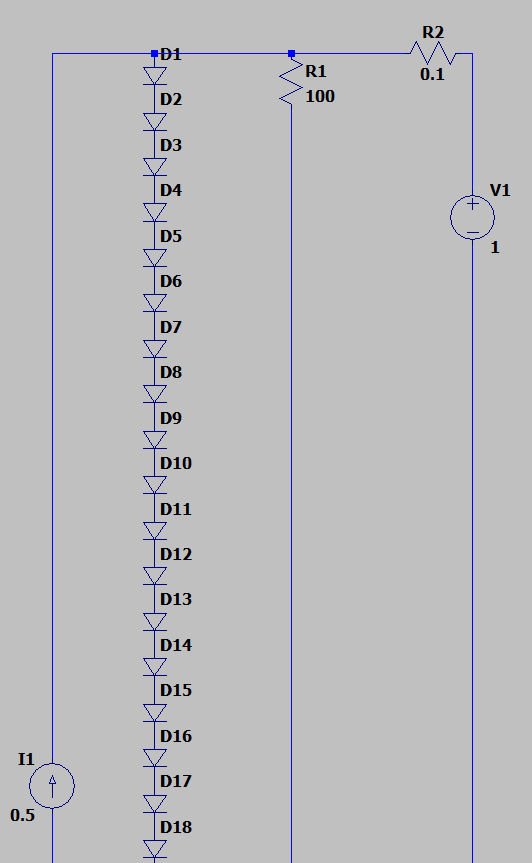
\includegraphics[width=0.5\textwidth]{Prework_images/LTSpice_cropped}
    	        	\caption{LTSpice circuit}
    	        	\label{fig:LTSpice}
    	        \end{figure}
    	       	\begin{figure}[H]
    	       		\centering
    	        	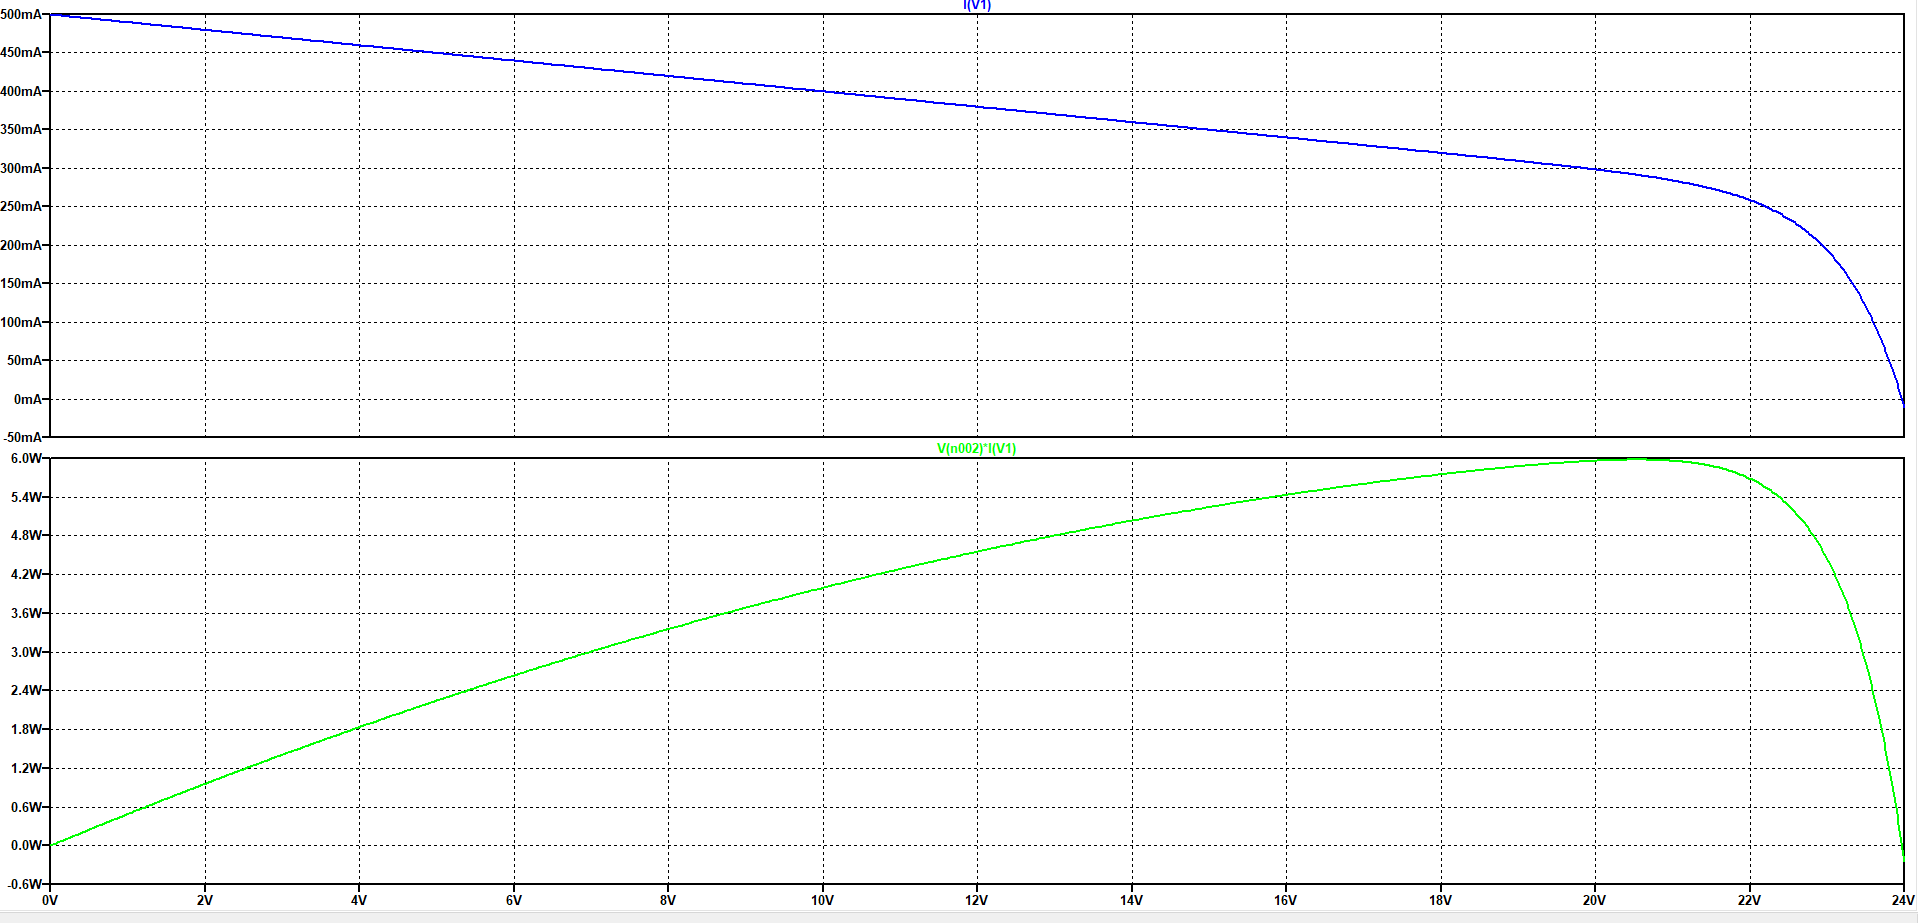
\includegraphics[width=\textwidth]{Prework_images/IVCurve}
    	        	\caption{I-V and P-V curves}
    	        	\label{fig:IVCurve}
    	        \end{figure}
    	    \subsubsection{Explain how the duty cycle should change to make the PV panel voltage constant and operate at the reference}
    	        If the PV panel voltage drops below the reference value, the duty cycle should be decreased in order to bring the voltage back to the reference value. Similarly, if the PV voltage rises above the reference value, the duty cycle should be increased to ensure the PV voltage drops to the reference voltage.
        
        \subsection{Lab Work}
            \subsubsection{PV Emulator}
                In order to properly implement the constant voltage reference MPPT algorithm, the maximum power point of the PV emulator was found by connecting the PV emulator in parallel with the lab power supply and connecting a variable resistance box to the circuit. The resistance was changed between $0\Omega$ and $270\Omega$ and the voltage and current were measured. Open circuit conditions were also measured. The results are shown in \cref{tbl:Lab3Emu}, and the I-V and P-V curves are shown in \cref{fig:Lab3IV,fig:Lab3PV}
                \begin{table}[H]
                    \centering
                    \begin{tabular}{|l|l|l|l|}
                        \hline
                        
                        Resistance & Current & Voltage & Power \\ \hline
                        0 & 0.412 & 0.22 & 0.09064 \\ \hline
                        1 & 0.411 & 0.7 & 0.2877 \\ \hline
                        4.7 & 0.411 & 2.17 & 0.89187 \\ \hline
                        10 & 0.411 & 4.34 & 1.78374 \\ \hline
                        22 & 0.41 & 9 & 3.69 \\ \hline
                        33 & 0.409 & 13.3 & 5.4397 \\ \hline
                        47 & 0.396 & 18.5 & 7.326 \\ \hline
                        68 & 0.313 & 20.9 & 6.5417 \\ \hline
                        100 & 0.208 & 20.9 & 4.3472 \\ \hline
                        220 & 0.095 & 20.9 & 1.9855 \\ \hline
                        245 & 0.085 & 20.9 & 1.7765 \\ \hline
                        270 & 0.077 & 20.9 & 1.6093 \\ \hline
                        O/C & 0 & 20.9 & 0 \\ \hline
                        
                        \end{tabular}
                        \caption{Electrical Characteristics of PV Emulator}
                        \label{tbl:Lab3Emu}
                    \end{table}
                    \begin{figure}[H]
                        \centering
                        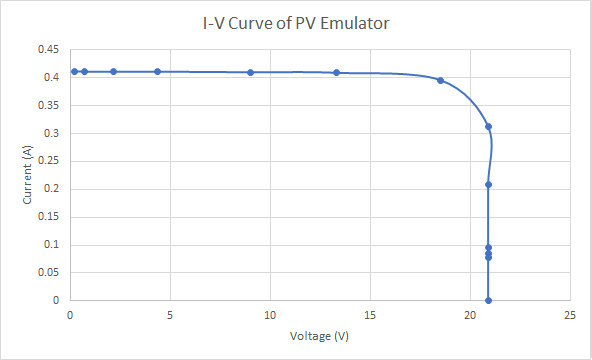
\includegraphics{Lab3Results/IVCurve}
                        \caption{I-V Curve of PV Emulator}
                        \label{fig:Lab3IV}
                    \end{figure}
                    \begin{figure}[H]
                        \centering
                        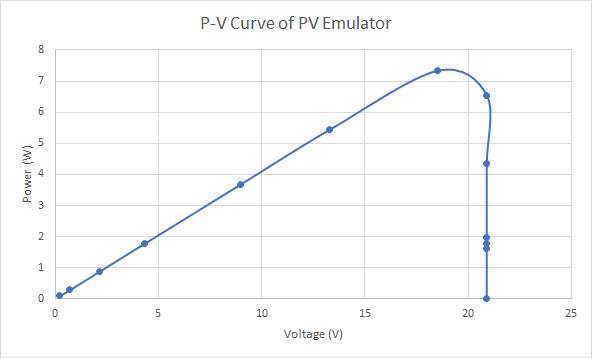
\includegraphics{Lab3Results/PVCurve}
                        \caption{P-V Curve of PV Emulator}
                        \label{fig:Lab3PV}
                    \end{figure}
            \subsubsection{Testing of Constant Voltage Reference MPPT}
                The lab's buck converter was connected between the PV emulator and the variable resistance box, and set up using an Arduino as the PWM driver. The lab power supply was set to 21V and the resistance box set to $33\Omega$. It was verified to be operating correctly, as shown in \cref{fig:lab3buck}.
                \begin{figure}[H]
                    \centering
                    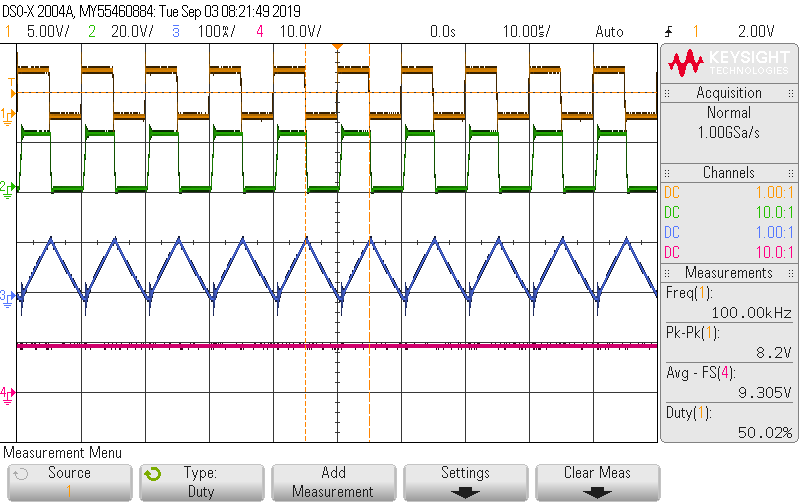
\includegraphics[width=0.75\textwidth]{Lab3Results/BuckTest_50DutyCycle_100KHz}
                    \caption{Correct operation of lab buck converter}
                    \label{fig:lab3buck}
                \end{figure}
                The MPPT algorithm could then be tested by varying the input current and measuring the output power. Oscilloscope captures showing the duty cycle of the buck converter, displayed in orange, power output of the buck converter, displayed in pink, the input current, displayed in blue, and output voltage, displayed in red, are shown in \crefrange{fig:Lab3_0.3A}{fig:Lab3_0.6A}
                \begin{figure}[H]
                    \centering
                    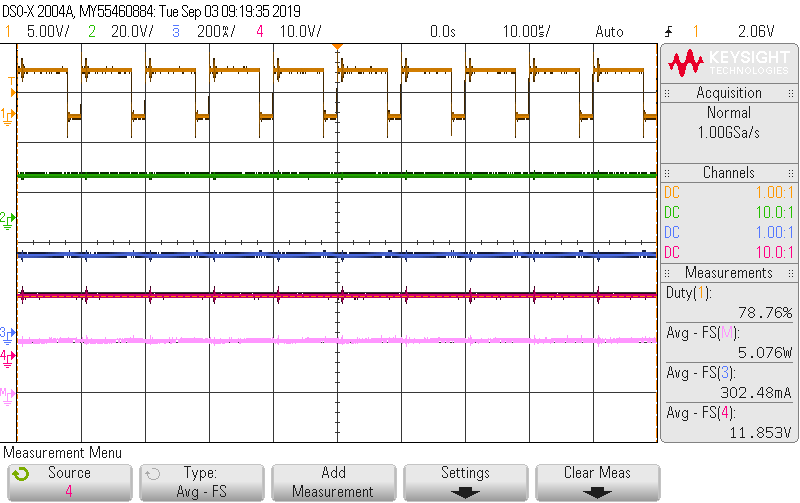
\includegraphics[width=0.75\textwidth]{Lab3Results/0_30A_Supply}
                    \caption{Constant Voltage Reference MPPT with 0.3A supply}
                    \label{fig:Lab3_0.3A}
                \end{figure}
                \begin{figure}[H]
                    \centering
                	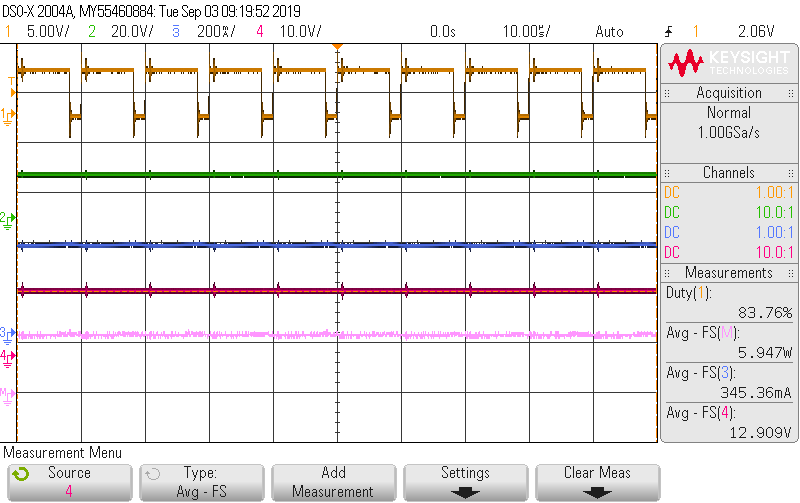
\includegraphics[width=0.75\textwidth]{Lab3Results/0_35A_Supply}
                    \caption{Constant Voltage Reference MPPT with 0.35A supply}
                    \label{fig:Lab3_0.35A}
                \end{figure}
                \begin{figure}[H]
                    \centering
                    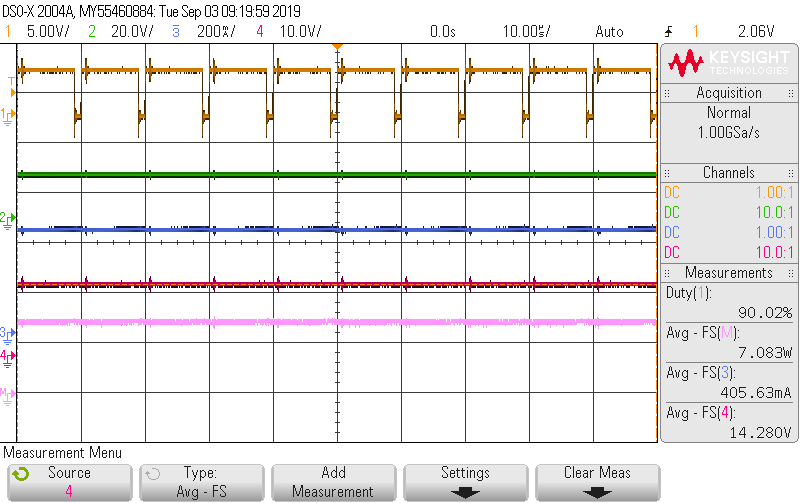
\includegraphics[width=0.75\textwidth]{Lab3Results/0_40A_Supply}
                    \caption{Constant Voltage Reference MPPT with 0.4A supply}
                    \label{fig:Lab3_0.4A}
                \end{figure}
                \begin{figure}[H]
                    \centering
                    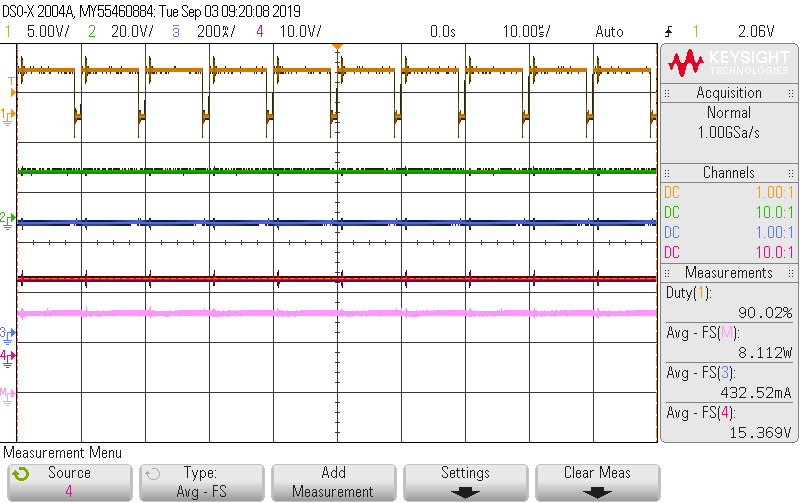
\includegraphics[width=0.75\textwidth]{Lab3Results/0_45A_Supply}
                    \caption{Constant Voltage Reference MPPT with 0.45A supply}
                    \label{fig:Lab3_0.45A}
                \end{figure}
                \begin{figure}[H]
                    \centering
                    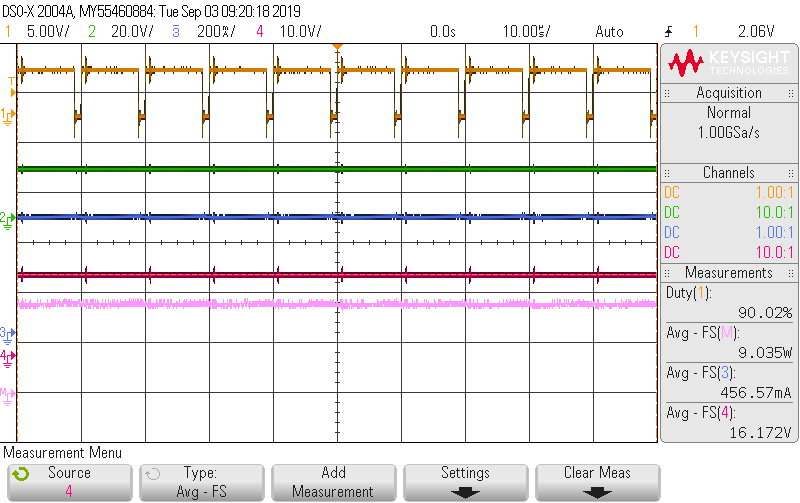
\includegraphics[width=0.75\textwidth]{Lab3Results/0_50A_Supply}
                    \caption{Constant Voltage Reference MPPT with 0.5A supply}
                    \label{fig:Lab3_0.5A}
                \end{figure}
                \begin{figure}[H]
                    \centering
                    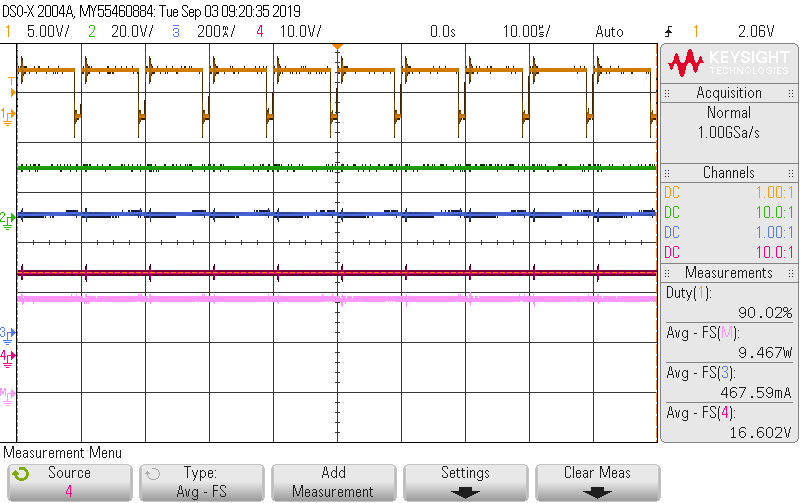
\includegraphics[width=0.75\textwidth]{Lab3Results/0_55A_Supply}
                    \caption{Constant Voltage Reference MPPT with 0.55A supply}
                    \label{fig:Lab3_0.55A}
                \end{figure}
                \begin{figure}[H]
                    \centering
                    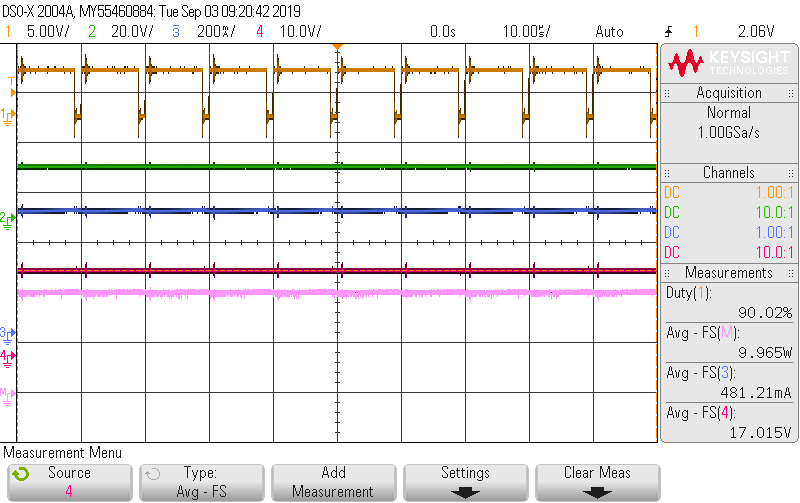
\includegraphics[width=0.75\textwidth]{Lab3Results/0_60A_Supply}
                    \caption{Constant Voltage Reference MPPT with 0.6A supply}
                    \label{fig:Lab3_0.6A}
                \end{figure}
   		\subsection{Analysis}
   			\subsubsection{Explain, with aid of equations and diagram, how the buck converter serves as a variable resistor to the PV panel}
   			\subsubsection{Explain your part of the code to achieve constant voltage reference MPPT with the support of experimental results}
   			\subsubsection{Compare the constant voltage reference MPPT performance against the identified true MPPs}
   	
   	\section{Perturb and Observe (P\&O) MPPT}
   	    \subsection{Pre-Work}
   	        \subsubsection{Explain why the power information at a particular point can be simplified to:   	        \\$\text{Power information at point } X = V_{out} \times V_{PV}$} \label{sssec:Powerinfo}
   	            The power of the PV panel is given by $P_{PV} = I_{PV} \times V_{PV}$, where $I_{PV}$ is the current and $V_{PV}$ is the voltage produced by the PV panel. As the current produced by the PV panel can be found by multiplying the circuit output current, $I_{out}$, by the duty cycle of the buck converter, $D$, the power equation can be represented as $P_{PV} = D I_{out} \times V_{PV}$. Using Ohm's Law, the equation can be further represented as $P_{PV} = D \frac{V_{out}}{R_{out}} \times V_{PV}$. As the P\&O algorithm does not need to take actual values into account, only their relative magnitudes, any constant values can be omitted and the power information can be represented as:
   	            \begin{equation*}
   	                \text{Power information at point } X = V_{out} \times V_{PV}
   	            \end{equation*}
   	            
	    	
	   	    \subsubsection{Design a Perturb and Observe Algorithm in Your Own Words}
	   	        The control system obtains the power information at a given point on the PV panel's P-V curve using the equation in \cref{sssec:Powerinfo} and stores it. The control system then reduces the buck converter's duty cycle and measures the power information at the new operating point. If the power at the new operating point is greater than the old operating point, the control system will continue to decrease the duty cycle when measuring the change. However, if the power information at the new operating point is less than that at the old operating point, the control system will increase the duty cycle. Once the power begins to drop again, the control system will start to decrease the duty cycle. This process happens continuously, ensuring the power output will oscillate around the maximum power point of the system.\\
	   	        
	   	        Overall, when the power drops when the duty cycle is increasing, the controller will switch to decreasing the duty cycle, and if the power drops while the duty cycle is decreasing, the controller will switch to increasing the duty cycle.
       
       \subsection{Lab Work}
   	    
   		\subsection{Analysis}
   			\subsubsection{Explain your part of the code to achieve P\&O MPPT with the support of experimental results}
   			\subsubsection{Compare the P\&O MPPT performance against the identified true MPPs}
   			\subsubsection{Is P\&O a perfect maximum power point algorithm? Why or why not? Explain your argument with the experimental results if possible}
   			\subsubsection{Suggest a way to improve the tracking accuracy of P\&O}
\end{document}

